% !TEX root = thesis.tex
\section{Open Source Code for Low Resource Languages}
\label{sec:lrl-code}

Now that low resource languages have been described, and now that there has been a brief overview of open source as a software methodology, the reader will doubtless wonder - what is the state of open source code that can be used today by LRL communities?

Due to the decentralised nature of open source, this is an inherently difficult question to answer. Nevertheless, there are a few strategies that can be used to approach an answer. In this chapter, I explore the following: 

\begin{itemize}
\item Section~\ref{subsec:mapping}: I use a specific task - making language maps using locationally tagged data -  as a case study for what tools might be used by language researchers;
\item Section~\ref{subsec:lrl-nlp-through-providers}: I look at what resources are available from any of the main large data aggregators mentioned in Section~\ref{subsec:resource-aggregators};
\item Section~\ref{subsec:lod}: I examine the Linked Open Data cloud for linguistic resources;
\item Section~\ref{subsec:popular-open-source-libraries}: I discuss projecting language resources across languages using open source software, \`a la \citet{bender2016linguistic}, and look at some of the more-cited open source tools used for LRL NLP;
\item Section~\ref{sec:solutions}: I sample relevant work on GitHub through a manually collected list of resources. 
\end{itemize}

A discussion of these strategies and the implications of their findings is presented in the summary in Section~\ref{subsec:lrl-summary}, as well as in Chapter~\ref{sec:discussion}.

\subsection{Case study: Mapping linguistic co\"ordinates}
\label{subsec:mapping}

Choosing a specific HLT task and then trying to perform that task as adequately as possible is one strategy for figuring out how much open source code exists, and what that looks like. There are cases where using open source software is decidedly simple. For instance, if the goal is to build a POS tagger using two hours of annotation, you could use the {\tt low-resource-pos-tagging-2014} package developed as part of \citet{garrette2013real,garrette2013learning}, and available on GitHub,\footnote{\href{https://github.com/dhgarrette/low-resource-pos-tagging-2014}{https://github.com/dhgarrette/low-resource-pos-tagging-2014}. \last{April~27}} under an Apache open license, without any other considerations than downloading Java and learning a bit of Scala, both free and open source languages. But this is a very limited use case, as this package was built as part of two scientific papers studying this narrowly scoped problem.

A more complex workflow will show the difficulties of using open source for low resource languages, and highlight what a research methodology might look like in depth. For example, suppose we were interested in making dialect maps using language co\"ordinates. This is an old research area in linguistics \citep{trudgill1983on,labov2005atlas}. Geolocationally-tagged language data has many useful applications. For instance, tagging tweets or text messages within a country can be used to understand dialects \citep{mubarak2014using}, or in crisis situations \citep{lewis2010haitian}. Geolocation can also be used to plot language relatedness \citep{littauer2012visualizing}.

Another example where geolocation might be useful outside of research would be in l10n in the browser. For instance, a client normally specifies what languages they use through ISO 639 tags,\footnote{\href{https://www.ietf.org/rfc/bcp/bcp47.txt}{https://www.ietf.org/rfc/bcp/bcp47.txt}. \last{April~27}} which are set automatically when they install their browser. If the client's browser does not send an {\tt Accept-Language} header\footnote{\href{https://tools.ietf.org/html/rfc7231\#section-5.3.5}{https://tools.ietf.org/html/rfc7231\#section-5.3.5}. \last{April~27}} with this information in their requests to view a website, then the server may use the {\tt Navigator\-Language} object in JavaScript\footnote{\href{https://www.w3.org/TR/html51/webappapis.html\#language-preferences}{https://www.w3.org/TR/html51/webappapis.html\#language-preferences}. \last{April~27}} to query for the language of the browser user interface. However, the server can also ask the client's browser directly through the Geolocation API (for instance, on Firefox\footnote{\href{https://www.mozilla.org/en-US/firefox/}{https://www.mozilla.org/en-US/firefox/}. \last{April~27}}\footnote{\href{https://developer.mozilla.org/en-US/docs/Web/API/Geolocation/Using_geolocation}{https://developer.mozilla.org/en-US/docs/Web/API/Geolocation/Using\_geolocation}. \last{April~27}}) to supply the geolocation of users and extrapolate plausible languages for the client. Knowing where the user is likely to be, and what languages the user is likely to prefer using, could help with providing their native language automatically in the browser.

\citet{gawne2016mapmaking} give a general overview of the mapping field currently, pointing out that the main resource for finding language geographical co\"ordinates comes from the World Language Mapping System (WLMS),\footnote{\href{http://www.worldgeodatasets.com/language/.}{http://www.worldgeodatasets.com/language/}. \last{April~25}} a website owned and run by SIL. The WLMS data is used to specify locations for ISO 639-3 labelling, and by Glottolog and OLAC. SIL's maps are under a closed license and must be purchased. \citet{gawne2016mapmaking} also mention WALS, which uses its own geographical co\"ordinates, and the ELP, which uses Google Maps as its mapping program,\footnote{Unsurprisingly, as the ELP is funded by Google.} and draws from multiple sources. They also mention Language Landscape,\footnote{\href{http://www.languagelandscape.org/}{http://www.languagelandscape.org}. \last{April~25}} a project which maps instances of language use.

To use these geographic information systems (GIS), one needs to download licensed map data, which could be open or closed. Then, one has to have a mapping software to display that data. This software must also be appropriately licensed. Google Maps is not open source, although it is {\it open access}, in that it is free to use. An open source equivalent of Google Maps is Open Street Maps,\footnote{\href{https://www.openstreetmap.org/}{https://www.openstreetmap.org/}. \last{April~27}} a community built tool that is permissively licensed as CC-BY-SA.\footnote{\href{https://www.openstreetmap.org/copyright}{https://www.openstreetmap.org/copyright}. \last{April~27}} One could use data from Glottolog and then provide a map using Open Street Map while using entirely open source applications, or one could use Google Maps with the same end result. The only difference between the two methodologies from an open source perspective is that the engine making Google Maps would be still be a proprietary black box.

It is this mixed use case that is most common - researchers or NLP practitioners use a mix of open and closed resources, as needed. \citet{gawne2016mapmaking} mention many programs: Google Earth\footnote{\href{https://www.google.com/earth/}{https://www.google.com/earth/}. \last{April~27}} (closed source, free) for base maps; Geotag\footnote{\href{http://geotag.sourceforge.net/}{http://geotag.sourceforge.net/}. \last{April~27}} (free, open source) and Photo KML\footnote{\href{http://www.visualtravelguide.com/Photo-kml.html}{http://www.visualtravelguide.com/Photo-kml.html}. This URL was provided in \citet{gawne2016mapmaking}, but may be down permanently.} (free) for accessing GIS embedded in pictures taken on iPhones (closed); the KML and KMZ formats,\footnote{\href{http://www.opengeospatial.org/standards/kml/}{http://www.opengeospatial.org/standards/kml/}. \last{April~27}} originally developed by Google for Google Earth but now standards implemented by the Open Geospatial Consortium\footnote{\href{http://www.opengeospatial.org}{http://www.opengeospatial.org}. \last{April~27}} and licensed openly and freely; Koredoko\footnote{\href{https://itunes.apple.com/us/app/koredoko-exif-and-gps-viewer/id286765236}{https://itunes.apple.com/us/app/koredoko-exif-and-gps-viewer/id286765236}. \last{April~27}} for viewing GIS data in photos (closed, free); CartoDB\footnote{\href{https://carto.com/}{https://carto.com/}. \last{April~27}} (proprietary) and CartoCSS\footnote{\href{https://github.com/mapbox/carto}{https://github.com/mapbox/carto}. \last{April~27}} (free, open); TileMill\footnote{\href{https://www.mapbox.com/tilemill/}{https://www.mapbox.com/tilemill/}. \last{April~27}} (free, open, but no longer maintained or updated) and MapBox\footnote{\href{https://www.mapbox.com/mapbox-studio/}{https://www.mapbox.com/mapbox-studio/}. \last{April~27}} (open, freemium\footnote{Meaning that certain features are free, while others require some sort of payment; a common way of funding open source projects.}) ; QGIS\footnote{\href{https://www.qgis.org/}{https://www.qgis.org/}. \last{April~27}} (free, open); the SQL\footnote{\href{https://www.iso.org/committee/45342/x/catalogue/p/1/u/0/w/0/d/0}{https://www.iso.org/committee/45342/x/catalogue/p/1/u/0/w/0/d/0}. \last{April~27}} language (free, open - languages and formats also have licensing laws and can be copyrighted\footnote{Constructed natural languages can also be licensed and copyrighted, leading to legal complications involving corporations suing fan communities for publishing documentation in a given language. Further discussion is well out of scope here, although the implications of language copyright do provide an interesting intellectual exercise.});
JPEG\footnote{\href{https://www.iso.org/standard/54989.html}{https://www.iso.org/standard/54989.html}. \last{April~27}} and PNG\footnote{\href{https://www.iso.org/standard/29581.html}{https://www.iso.org/standard/29581.html}. \last{April~27}} image formats (free, open); Adobe PhotoShop\footnote{\href{https://www.adobe.com/products/photoshop.html}{https://www.adobe.com/products/photoshop.html}. \last{April~27}} (closed source, paid); and CartoHexa\footnote{\href{https://www.colorhexa.com/}{https://www.colorhexa.com/}. \last{April~27}} (free, closed), among others that I may have missed.

It may be useful to look only at a specific part of the research methodology used in \citep{gawne2016mapmaking} in order to highlight more clearly what a mixed workflow looks like. One such example would be where they use a closed source application or website to shim (transfer from one format to another) open source data, as below:

\begin{quote}
To give some more general locational context we downloaded some Open Access geopolitical boundaries for Nepal from the Global Administrative Areas website.\footnote{\href{https://gadm.org/download}{https://gadm.org/download}. \last{April~27}} This data was downloaded as KMZ, which TileMill cannot read, so we opened the files in Google Earth (remember ... that KMZ is a compressed KML) and resaved them as KML, which TileMill can read. \citep[228]{gawne2016mapmaking}
\end{quote}

Here, they used Google Earth, which is closed source, to deal with open sourced data. There are open source alternatives for converting KMZ to KML. A cursory look on GitHub shows 54 repositories that could be relevant,\footnote{\href{https://github.com/search?p=1&q=kmz+kml&type=Repositories}{https://github.com/search?p=1\&q=kmz+kml\&type=Repositories}. \last{April~27}} including one which does solely this task (albeit with Spanish documentation).\footnote{\href{https://github.com/fadamiao/kmz2kml}{https://github.com/fadamiao/kmz2kml}. \last{April~27}}

Dogmatically using an entirely open source pipeline for working with language (or GIS data, as here) is rare, although it is hypothetically possible. However, one quickly runs into problems with this approach, as each subsequent layer of computational processing must then depend upon open source - including the operating system (for instance, GNU/Linux as an open source alternative to the closed Mac OS), processor, silicon chips, and so on. Or consider that GIS data often depends upon GPS co\"{o}rdinates. The Global Positioning System is run by the US Air Force, and owned by the US Government, and the systems which run it are almost certainly closed source for security reasons. At what level, then, can a workflow be judged to be open source or not?

By using {\it reductio ad absurdum}, it is easy to see that using both open source and closed source tools is more manageable. This is one of the reasons that copyleft remains an issue in licensing, as it enforces open source for all subsequent code, forcing one particular methodology at the expense of ease of use. However, open source tools have a certain flexibility for usage, in that they can be modified, shared, reused, and integrated more easily than so-called `black box' programs which do not proffer up information on how they work. 

\citepos{gawne2016mapmaking} suggestions for mapping use many closed, black-box applications. However, different studies show how to achieve similar results using entirely open source tools on the web. As \citet{hu2012multimedia, hu2018web} notes, the general trend in mapping software has been away from native applications\footnote{`Native' here means built for an operating system; not indigenous as in language communities.} and towards web applications, which may have a steeper learning curve, but which afford remote storage and access, and user access over the Internet. WALS uses LeafletJS,\footnote{\href{https://leafletjs.com/}{https://leafletjs.com/}. \last{April~26}} an open source mapping software that uses Open Street Maps as an alternative to using an embedded Google Maps map using their API. \citet{hu2018web} suggests a workflow that uses Leaflet along with jQuery,\footnote{\href{https://jquery.com/}{https://jquery.com/}. \last{April~26}} an open source JavaScript utility library, to display GIS linguistic maps. Web applications can also be used to display geographical data for research; \citet{littauer2013linguistic}, for instance, explored using a SPARQL endpoint to mine RDF data, including geographic location from WALS, to map Dogon languages using Open Street Maps. Here, we see that open source tools do exist for the use case of making dialect maps for language co\"ordinates. 

On a related note, is also important to open source the code used for the research in a paper, not just to use open source tools to achieve a desired product. For instance, \citet{cenerini2017mapping} cite several open source software applications and libraries they used in their study mapping the Cree-Innu-Naskapi continu\"{u}m using data from the Algonquian Linguistic Atlas \citep{junker2011linguistic},\footnote{\href{http://www.atlas-ling.ca/}{http://www.atlas-ling.ca/}. \last{April~26}} but do not open source their own code. This would have been useful, specifically as replicating their study using R \citep{ihaka1996r} would require researchers to write all of their own queries again. More on data privacy in academia is discussed in Section~\ref{subsec:data-and-privacy}.

The above is a small example, looking at only a couple of papers and showing how following open source methodology can be difficult, and how using mixed source applications is often the status quo. This is a single use case, and every application involving NLP requires navigating software and licensing laws. My purpose in providing this study is to point out how describing the state of open source code that could be used for LRLs is not clear cut. 

One could argue that this case is reflective of linguistic software, as opposed to NLP or computational linguistics. This arbitrary division is not useful, as all actors using language data that has been digitally encoded fall under the wider umbrella of users of human language technology. Languages do not exist within a vacu\"{u}m, and computational linguists using NLP to run deep learning artificial intelligence algorithms on spoken language corpora at scale depend upon previous work done by linguists, language communities, and researchers who spent time on the ground formalising orthographies, compiling dictionaries, and debating the finer points of linguistic minutiae.

\subsection{LRL NLP available through data providers}
\label{subsec:lrl-nlp-through-providers}

Another strategy is to look at the databases where NLP practitioners, researchers, and language activists find code for their respective languages directly. Using the list of aggregators from Section~\ref{subsec:resource-aggregators}, it is possible to give a general overview of what is available.

\subsubsection{Few to no computational resources}

Finding code resources is not easy. Many aggregators simply do not profile code resources at all. The Endangered Languages Project, for instance, contains information on over 3000 languages, and catalogues 6830.\footnote{\href{http://www.endangeredlanguages.com/resources/}{http://www.endangeredlanguages.com/resources/}. \last{April~24}} None of these resources are code. The searchable formats are: Format, Image, Video, Document, Audio, Link, and Guide. Glottolog only has academic references, and ODIN only has interlinear glossed text (IGT) corpora. Omniglot describes alphabets but does not index tooling for them. CLARIN has thousands of resources - but none of them are code, and you need to be an accredited researcher from a European institution to access them. The ELRA site provides hundreds of corpora resources - for purchase. The LRE Map\footnote{\href{http://www.resourcebook.eu/searchll.php}{http://www.resourcebook.eu/searchll.php}. \last{April~27}} is incredibly promising, in that it has around two thousand resources which are searchable; however, there are no links provided to any resource, and the accessibility or licensing of these resources is not listed. The language search functionality is currently not functioning, and the data is not machine accessible.\footnote{As of April~27, 2018.}

\subsubsection{Some scoped computational resources}

Some aggregators have more scoped suggestions for tooling. The first resource aggregator listed in Section~\ref{subsec:resource-aggregators} starts on the lower end of the language resource pyramid: Unicode's CLDR resources. Unicode is often the first port-of-call for a language team working on developing scripts for their language, unless the script is already using some  pre\"{e}xisting format (such as the Roman alphabet). CLDR has instructions on checking out their open source Subversion\footnote{\href{https://subversion.apache.org/}{https://subversion.apache.org/}. \last{May~3}} repository online.\footnote{\href{http://cldr.unicode.org/index/downloads}{http://cldr.unicode.org/index/downloads}. \last{April~24}} They also have a GitHub repository\footnote{\href{https://github.com/unicode-cldr/cldr-json}{https://github.com/unicode-cldr/cldr-json}. \last{April~24}} and organisation with code for digesting the normally XML representation in JSON, the notation format used most often by JavaScript developers. However, CLDR is not an aggregator - it is more of a suite of tools under one umbrella, as the scope is limited to working with the Unicode format.

OLAC, with hundreds of thousands of resources, has a tooling page,\footnote{\href{http://www.language-archives.org/tools.html}{http://www.language-archives.org/tools.html}. \last{April~26}} which mainly helps with working with OLAC as opposed to pointing to resources which can be used with language data. Unfortunately, searching for software resources comes up short. A short look at a specific language, Nask\-api, shows 23 resources,\footnote{\href{http://www.language-archives.org/language/nsk}{http://www.language-archives.org/language/nsk}. \last{April~26}} most of which are published papers - except for An Cr\'ubad\'an's archive, the Glottolog reference, typological references on WALS and on the Rosetta Project, and a link to resources noted on the LINGUIST List, which lists no resources when accessed.\footnote{\href{https://linguistlist.org/olac/search-olac.cfm?LANG=nsk}{https://linguistlist.org/olac/search-olac.cfm?LANG=nsk}. \last{April~26}} Scottish Gaelic is not much different (26 resources),\footnote{\href{http://www.language-archives.org/language/gla}{http://www.language-archives.org/language/gla}. \last{April~26}} although it does point to some corpora.

The Linguistic Data Consortium has a tool page,\footnote{\href{https://www.ldc.upenn.edu/language-resources/tools}{https://www.ldc.upenn.edu/language-resources/tools}. \last{April~26}} where it notes five tools that may be useful for researchers using its data. These tools are Annotation Graph Kit (AGTK), the Champollion Toolkit, the LDC Word Aligner, Sphere Conversion tools, and XTrans, of which only Sphere has a non-standard open license that allows use but may have more restrictions. This suite of tools is particularly useful for dealing with LDC data. This sort of tool and corpus bundling is common; when building a resource, the tools to manage that resource are included directly in a tools page. DOBES has the same type of page,\footnote{\href{http://dobes.mpi.nl/archive_info/tools/}{http://dobes.mpi.nl/archive\_info/tools/}. \last{April~26}} where they mention tools developed at The Language Archive: ELAN, a powerful tool for time aligned annotation of video or audio data; ARBIL, a metadata catalogue creation tool; LAMUS, a tool for uploading data and metadata into the DOBES archive and for managing existing collections; and LEXUS, a web-based lexicon tool. 

For field linguistics, the mixture of apps and small tooling is common, as is combining corpora with tools in some fashion. For instance, \citet{caballero2017choguita} presents a fieldwork paper on Choguita Rar\'amuri (Tarahumara), an Uto-Aztecan language. In the paper, they mention using Microsoft Word\footnote{\href{https://products.office.com/en-CA/word}{https://products.office.com/en-CA/word}. \last{April~26}} and Excel,\footnote{\href{https://products.office.com/en-CA/excel}{https://products.office.com/en-CA/excel}. \last{April~26}} SIL's Fieldwork Language Explorer (FLEx),\footnote{\href{http://software.sil.org/fieldworks/download/.}{http://software.sil.org/fieldworks/download/}. \last{April~26}} and show screenshots of Quicktime.\footnote{\href{https://support.apple.com/quicktime}{https://support.apple.com/quicktime}. \last{April~26}} The corpus they present is stored on the Endangered Language Archive at SOAS, University of London\footnote{\href{elar.soas.ac.uk/deposit/0056}{elar.soas.ac.uk/deposit/0056}. \last{April~26}} \citep{caballero2009data}. The majority of these tools are closed source, except for FLEx. However, they also mention using ELAN.\footnote{\href{https://tla.mpi.nl/tools/tla-tools/elan/}{https://tla.mpi.nl/tools/tla-tools/elan/}. \last{April~26}} \citet{caballero2017choguita} made their own tools to work with ELAN, and they made this code available on GitHub.\footnote{\href{https://github.com/ucsd-field-lab/kwaras}{https://github.com/ucsd-field-lab/kwaras}. \last{April~26}} In order to access the data, the reader is likely to have read the paper; thus the document, the code, and the corpus together form a unit of research, which are all used together.

\subsubsection{Many computational resources}

The low number of suggested tools above (less than a dozen, in most cases) is not unusual, but there are some archives that have more tools listed. For instance, the Resource Network for Linguistic Diversity (RNLD), a largely Australian network, lists dozens of tools and applications that could be useful.\footnote{\href{http://www.rnld.org/software}{http://www.rnld.org/software}. \last{April~26}} The list does not differentiate between bundled code that works as native applications, and code which must be downloaded and run through a terminal. EMELD, the Electronic Metastructure for Endangered Languages Data (a five-year project run through LDC, the ELF, and the Universities of Arizona, Eastern Michigan, and Wayne State) has a similar list with hundreds of items.\footnote{\href{http://emeld.org/school/toolroom/software/software-display.cfm}{http://emeld.org/school/toolroom/software/software-display.cfm}. \last{April~26}}

META-SHARE, which aggressively pursues open access and open licensing for resources in its database, has 344 tools available, and allows easy searching for these tools,\footnote{\href{http://www.meta-share.org/}{http://www.meta-share.org}. \last{April~26}} although signing up as a user is necessary. The ACL Wiki has resources for 84 languages.\footnote{\href{https://aclweb.org/aclwiki/List_of_resources_by_language}{https://aclweb.org/aclwiki/List\_of\_resources\_by\_language}. \last{April~26}} From a random selection of these resources (including corpora), one could get an idea of how many resources are totally aggregated: Arabic (16), Navajo (1), Catalan (8), Faroese (4), Galician (20), Maltese (4), Irish (10). However, the quality is not assured. Many links point to the same tools which are used cross-linguistically, or do not resolve altogether. LT-World lists 523 separate tools (this number was reached by adding up all resource amounts listed on their language tools page\footnote{\href{http://www.lt-world.org/kb/resources-and-tools/language-tools/}{http://www.lt-world.org/kb/resources-and-tools/language-tools}. \last{April~26}} and assuming that there is no duplication of tools, which may be inaccurate). These tools are for all languages, and only a subset could be understood to apply to LRLs.

\subsubsection{Summary of computational resources}

These collected resources are, to my knowledge, the main places to look for aggregated data around software resources on particular languages. From this, it is clear that there are global open source software resources in the order of hundreds, not thousands. Considering that thousands of languages have not ascended digitally, this is not ideal. There is clearly more work which can be done to make resources available and accessible, particularly for LRLs.

\subsection{Linked open data}
\label{subsec:lod}

The aggregators mentioned in Section~\ref{subsec:lrl-nlp-through-providers} are largely massive databases which store corpora on their own servers, or are HTML pages that linked directly to other resources using hardcoded links. OLAC is an exception; it uses an XML representation of the Dublin Core metadata set \citep{dublin1998dublin}, and uses infrastructure based on the Open Archives Initiative's Protocol for Metadata Harvesting (OAI-PMH).\footnote{\href{http://www.openarchives.org}{http://www.openarchives.org}. \last{April~26}} OLAC uses a protocol on top of this to pool resources from many sources; resources which wish to be entered need to have metadata which conforms to a certain standard, and then they can be aggregated \citep{simons2001olac}. The CLARIN VLO \citep{mccrae2015one} also uses the OAI-PMH protocol \citep{sompel2004resource, mccrae2015reconciling}. These two providers of data do not share data with each other automatically. Any resource added to one will not automatically be added to the other, even though they use the same protocol. Isolated data is a persistent problem across the aggregators, as data which exists in independent silos makes accessing, searching, and updating data difficult for both users and data administrators.

Linghub and the Linguistics Linked Data cloud were both created to resolve this issue of data siloization. The latter is a linked data ontology created by the Open Linguistics Working Group (OWLG) \citep{chiarcos2011working, chiarcos2012open, chiarcos2013building, mccrae2016open}, largely by manually selecting linguistic data sources from Datahub.io for aggregation. The Linguistic Linked Open Data (LLOD) cloud \citep{chiarcos2012linking} can be previewed at \href{http://linguistic-lod.org}{\nolinkurl{http://linguistic-lod.org}},\footnote{\href{http://linguistic-lod.org/}{http://linguistic-lod.org}. \last{April~26}} and in Figure~\ref{fig:llod}.

\begin{figure}
 \centering
 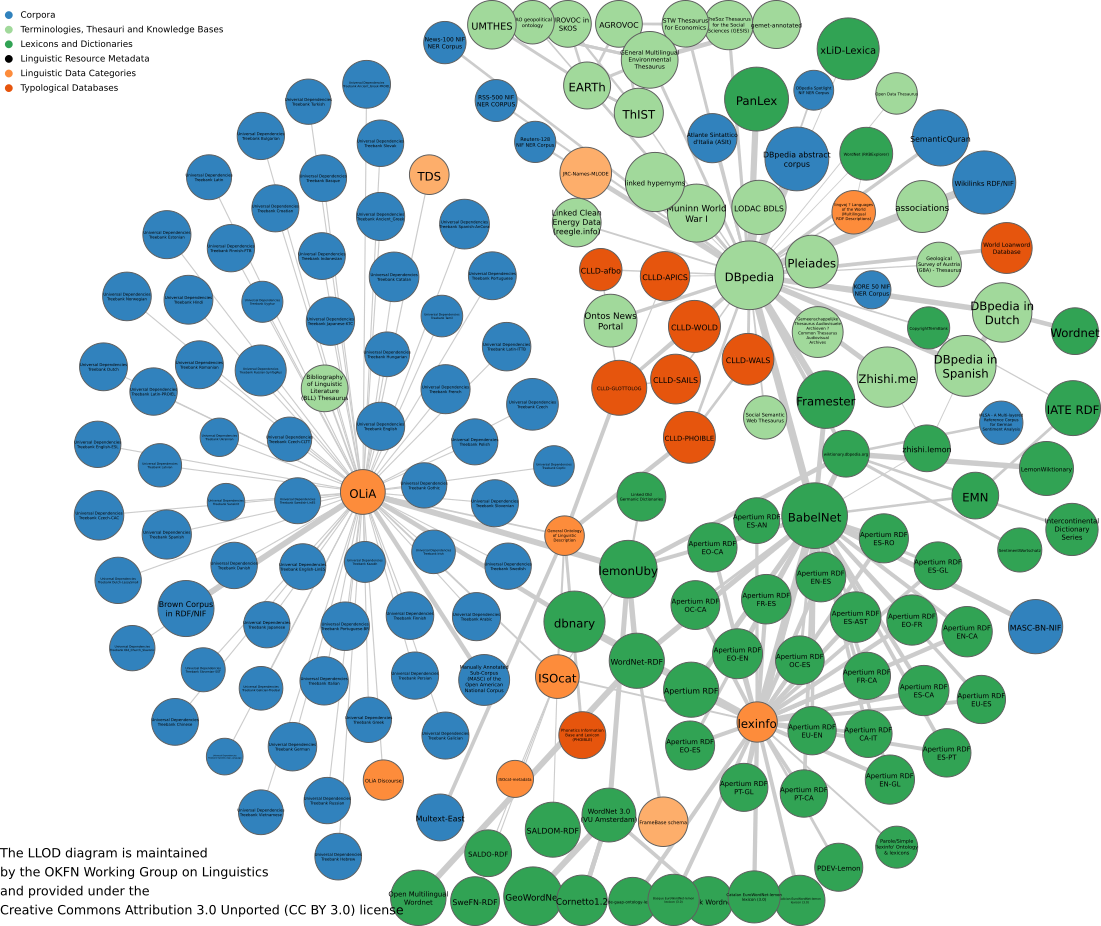
\includegraphics[width=1\textwidth]{img/llod.png}
 \caption{The most recent Linguists Linked Open Data cloud from \href{http://linguistic-lod.org}{http://linguistic-lod.org} (Described in \citet{chiarcos2012linking})}
 \label{fig:llod}
\end{figure}

Linghub \citep{mccrae2015linghub, mccrae2015reconciling} was created to allow for mining of all available databases - including META-SHARE, LRE Map, Datahub, and CLARIN's VLO - using SPARQL, a query language that works for Semantic Web ontologies encoded in RDF. Since \citet{mccrae2015linghub} was published, OLAC has allowed its resources to also be mined.\footnote{\href{http://www.language-archives.org/news.html\#llod}{http://www.language-archives.org/news.html\#llod}. \last{April~26}} At this point, there are few large repositories of language resource data which are unable to be queried. However, linked data has the existential failing of only including metadata which has been included in the available data sources. It is a fantastic resource for finding corpora, and \citet{mccrae2015linghub} gives several examples of finding data through the cloud;  it is also an exceptional way to mine the LRE map database, which provides names of language resources for NLP tooling. But there is a barrier to entry of learning SPARQL and using an available portal, and any work outside of the curated, largely academic resources may not be available.

The linked open data cloud and Linghub also do not explicitly cater to LRLs, although there has been some work in this area. \citet{huang2017linking} used basic lexicons, such as the Swadesh list \citep{swadesh1955towards} of common words used in lexically dating languages, to automatically develop ontologies of cultural knowledge for LRLs. While this does not provide better coverage of language resources, ontologies can be useful themselves for translation and searching lexicons. A more detailed use case for automatically linking LRLs could be attempted, for instance by scraping the internet for pages that use the language (similar to An Cr\'{u}bad\'{a}n) and automatically adding those to the LOD. More work in this area is needed.

\subsection{Multilingual NLP libraries}
\label{subsec:popular-open-source-libraries}

While searching for code that has been tagged with metadata noting the language it serves has some merits, there are also possibilities for using generic code on many languages. For instance, \citet{bender2016linguistic} explores the field of multilingual NLP (now decades old; for instance, \citet{kay1997proper} called for this in the 90s), pointing out that there is a growing body of research that uses language typology to abstract and identify language features which allow for applying NLP systems from one language to another.

\begin{quote}
Businesses developing commercial products with NLP are interested in the markets represented by {\tt low resource languages} (LRLs; i.e., those languages for which there are not many digitized data sets or basic NLP systems such as part-of-speech taggers or morphological or syntactic parsers), some of which represent very large populations in emerging economies. Finally, researchers looking to apply NLP techniques to assist in LRL documentation are naturally interested in developing NLP systems that work across very diverse languages.\citep[646]{bender2016linguistic}
\end{quote}

\citet{bender2016linguistic} goes on to mention the LinGo Matrix system \citep{bender2002grammar, drellishak2005coordination} that can be used to create rule-based grammars for natural languages using linguistic typographical data. The LinGo Matrix, and all work within the DELPH-IN system (a collaboration looking mainly at the Head-Driven Phrase Structure Grammar and Minimal Recursion Semantics) is open source.\footnote{\href{http://www.delph-in.net/wiki/index.php/Software}{http://www.delph-in.net/wiki/index.php/Software}. \last{April~26}}

They also mention projecting resources across languages, such as \citepos{yarowsky2001inducing} projections of linguistic annotations like POS tags and noun phrase parsing from English to French and Chinese, by using bilingual texts that had been word-aligned. This was extended in the previously mentioned \citet{agic2015if}, who used similar POS tagger projection for one hundred LRLs. Their code is open source on Bitbucket.\footnote{\href{https://bitbucket.org/lowlands/}{https://bitbucket.org/lowlands/}. \last{April~26}}

This avenue of research is fascinating and broad, because it allows for small tools to be applied to other LRLs at a minimal cost. A study involving looking at all of the available research, with an in-depth look in each scientific article that includes links to source code, would be warranted and welcomed. It is unfortunately largely out of scope for this thesis; it is enough, here, to know that open source code for LRLs is dependent upon academics working in this field sharing their code on large repositories, and that this code must also be adapted to each particular LRL, which, while an extensive task, is made easier through multilingual NLP and cross-linguistic projection.

At a lower level, there are language agnostic NLP toolkits which are useful for working with LRL datasets. The most well known is arguably the Natural Language Toolkit (NTLK)\footnote{\href{http://www.nltk.org/}{http://www.nltk.org/}. \last{April~26}} \citep{bird2006nltk}, a free and open source Python library that enables users to interface with over fifty different corpora and lexical resources, and which provides a suite of tools such as tokenizers and parsers which can be used in sparse data contexts. A primer \citep{bird2009natural}\footnote{Available online at \href{http://nltk.org/book}{http://nltk.org/book}. \last{April~26}} is used frequently in natural language processing classes written by the creators. It is licensed under the Apache 2.0 license, an open source license. \footnote{\href{https://github.com/nltk/nltk/blob/develop/LICENSE.txt}{https://github.com/nltk/nltk/blob/develop/LICENSE.txt}. \last{April~26}} On GitHub, there are currently 204 contributors listed,\footnote{\href{https://github.com/nltk/nltk/graphs/contributors}{https://github.com/nltk/nltk/graphs/contributors}. \last{April~10}} and the contribution history in Git shows 234 (found by using the command {\tt git authors}). Some of the resources within NLTK work especially well with LRLs. For instance, in 2015, NLTK added machine translation libraries, including popular ones such as IBM Models 1-3 and BLEU.

By open sourcing their code, the NLTK authors have allowed it to be adapted and re-used. Currently, there are several ports, or reimplementations in another programming language which allows use in different coding language ecosystems. One of these is the JavaScript language implementation.\footnote{\href{https://github.com/NaturalNode/natural}{https://github.com/NaturalNode/natural}. \last{April~26}} This has 6700 stars on GitHub, which, since they reflect favouritism from individual users, is a good indicator of community vitality and use, and 88 contributors. The port is also open source, under an MIT license.\footnote{\href{https://github.com/NaturalNode/natural\#license}{https://github.com/NaturalNode/natural\#license}. \last{April~26}}

It is difficult to track usage of these open source software packages by LRL communities or researchers, as, once downloaded, there are no convenient metrics which lead back to the original source. Code, when run, generally leaves no trace. Again, the fundamental problem of tracking LRL open source software inhibits understanding the ecosystem, but it is clear from individual anecdotes and through scientific citations that work is being done in this area.

\subsection{A GitHub database for open source code}
\label{sec:solutions}

Here, I present a curatorial, crowd-sourced database of language resources. This database has a mild advantage over Linghub and other large databases in that it is decentralised, easily accessible and readable without learning a new query language, and has a lower barrier to data entry.

Presented first in \citet{CCURL}, {\tt low-resource-languages} is a list of code resources for LRLs available on GitHub, available (under my namespace) at \href{https://github.com/RichardLitt/low-resource-languages}{https://github.com/RichardLitt/low-resource-languages}.\footnote{This was formerly called {\tt endangered-languages}. It was renamed to reflect attitudes mentioned in Section~\ref{subsubsec:response}.} The list is structured in Markdown,\footnote{\href{https://daringfireball.net/projects/markdown/syntax}{https://daringfireball.net/projects/markdown/syntax}. \last{April~26}} a lightweight format for text that is rendered natively on GitHub and is an industry standard in open source for structuring text documents.

Instead of using an XML or RDF representation that needs to be shown through a portal, this list natively works as a text list, although the metadata does not lend itself to aggregation in the same fashion as linked data. Making a scraper that would automatically translate the data into XML would be trivial. However, the benefit of using Markdown is that anyone on GitHub can easily parse and analyse the data directly, and that anyone can access and submit patches to add to the list. On GitHub, social coding conventions surrounding patches - called {\it pull requests} - allows for easy quality assurance of the data, as anyone suggesting an addition or deletion has to wait for a code maintainer to verify that their contribution is up to standard. This allows for a curated, collaborative approach to documentation and metadata aggregation. Curation occurs largely through my acceptance of related pull requests, along with other maintainers of the list - currently, Hugh Patterson of SIL,\footnote{\href{https://github.com/HughP}{https://github.com/HughP}. \last{April~26}} @cesine\footnote{\href{https://github.com/cesine}{https://github.com/cesine}. \last{April~26}} and @AnnaLuisaD of the Living Tongues Institute.\footnote{\href{https://github.com/AnnaLuisaD}{https://github.com/AnnaLuisaD}. \last{April~26}}

There are 441 links available in the list,\footnote{This figure was calculated by running \texttt{grep "\textbackslash* \textbackslash[" README.md | wc -l}.} with hundreds of general resources and 32 different subsections available for specific low resource languages. Instead of tagging resources directly, they are placed in single sections that best describe the resource. The language specific sections are for: Albanian, Alutiiq, Amharic, Arabic, Bengali, Chichewa, Galician, Georgian, Guarani, Hausa, Hindi, H\o gnorsk, Inuktitut, Irish, Kinyarwanda, Lingala, Lushootseed, Malay, Malagasy, Manx, Migmaq, Minderico, Nishnaabe, Oromo, Quechua, Sami, Scottish Gaelic, Secwepemcts\'in, Somali, Tigrinya, Yiddish, and Zulu. Other sections cover: Single language lexicography projects and utilities, Utilities, Software, Keyboard Layout Configuration Helpers, Annotation, Format Specifications, i18n-related Repositories, Audio automation, Text-to-Speech
Text automation, Experimentation, Flashcards, Natural language generation, Computing systems, Android Applications, Chrome Extensions, FieldDB, FieldDB Webservices / Components / Plugins, Academic Research Paper Specific Repositories, Example Repositories, Language \& Code Interfaces, Fonts, Corpora, Organizations On GitHub, Other OSS Organizations, and Tutorials. An overhaul of these sections would most likely be warranted, but there has been no general demand for this as of yet.

To date, there are 19 authors as recorded through {\tt git authors}, and 17 contributors recorded through GitHub's contributor view.\footnote{\href{https://github.com/RichardLitt/low-resource-languages/graphs/contributors}{https://github.com/RichardLitt/low-resource-languages/graphs/contributors}. \last{April~26}} Most pull requests came from @cesine, followed by @HughP. Six users contributed more than two pull requests. This data\footnote{\href{https://gist.github.com/RichardLitt/e60bcf9f399939b16181bf25ad6da8ba}{Available at https://gist.github.com/RichardLitt/e60bcf9f399939b16181bf25ad6da8ba}. \last{April~26}} came from an analysis of contributions using the GitHub API by using the {\tt name-your-contributors}\footnote{\href{https://github.com/mntnr/name-your-contributors/}{https://github.com/mntnr/name-your-contributors/}. \last{April~27}} tool, by running {\tt name-your-contributors -u RichardLitt -r low-resource-languages}.

A large majority of these files were last touched by me,\footnote{This figure was calculated by running {\tt git blame README.md | grep "Richard" | wc -l}.} as I have frequently reorganised and edited the list. In the past two weeks, GitHub's traffic shows 217 views by 37 unique visitors.\footnote{\href{https://github.com/RichardLitt/low-resource-languages/graphs/traffic}{https://github.com/RichardLitt/low-resource-languages/graphs/traffic}. \last{April~26}} There are a total of 39 forks, which reflects users who have copied the code to their own namespace (necessary for suggesting changes back to the main {\tt master} branch in GitHub). There are 166 stars and 24 watchers as of this writing.

An example entry is provided below, for {\tt fast\_align} \citep{dyer2013simple}. The syntax of the example is as follows: A bullet point to place the item in a list; A link within brackets pointing to the GitHub repository where the open source code is stored, or to the resource elsewhere; and a basic description taken from the repository.

\begin{quote}
{\tt * [fast\_align](https://github.com/clab/fast\_align) - Simple, fast unsupervised word aligner.}
\end{quote}

In \citet{CCURL}, we described how the list is aimed at project managers, community developers doing language development, linguists, and software developers, mentioning some cases where developers reached out to say thank you for the list. To summarise our description: the list is for everyone, and the ease of accessibility of GitHub and rendered Markdown make it suitable for any audience. We did not then highlight how being on GitHub is of paramount importance. It is GitHub's social platform, and their extensive community, which makes this list most relevant. Since most open source code is on GitHub, then it follows that facilitating discovery by putting metadata directly on the site is useful step to undertake. As well, since the code is in an open source Git repository, it is entirely possible for someone to easily copy the list and continue development and curation if for any reason my own copy goes down for any reason.

At LREC 2016 in Portoro\v{z}, where \citet{CCURL} was presented during the poster session\footnote{In reality, I presented it from my laptop as a way of facilitating input and discussion, as I felt that the analog quality of a poster would not properly convey the usefulness of the list, and as it was difficult to physically source a poster while hitchhiking from Italy.}, I collected responses on a Google Form from attendees (similar to data sourcing for LRE Maps, in some ways). There were 18 respondents. All but one of them said they have code related to LRLs; only six of them had GitHub accounts (although one more had a Bitbucket account). Some of them have since contributed to the list.

There were at least two complaints; one of list quality, and another that the pages and subpages are often dead. The second concern has been fixed by implementing {\tt awesome\_bot},\footnote{\href{https://github.com/dkhamsing/awesome_bot}{https://github.com/dkhamsing/awesome\_bot}. \last{April~26} I am also using this tool to verify and validate all links in this thesis.} a tool which automatically checks all of the links and ensures that they resolve, and continuous integration tests with it through TravisCI.\footnote{\href{https://travis-ci.org/RichardLitt/low-resource-languages}{https://travis-ci.org/RichardLitt/low-resource-languages}. \last{April~26}} I have also cloned all of the Sourceforge repositories into GitHub repositories, to ensure that the open source licensed code is available in the GitHub ecosystem.

\citet[88]{mccrae2015linghub} note that there are multiple ways of collecting metadata around resources, which provide their motivation to combine different collections built using different strategies in Linghub. 

\begin{quote}
Currently, two approaches to metadata collection for language resources can be distinguished. Firstly, we distinguish a curatorial approach to metadata collection in which a repository of language resource metadata is maintained by a cross-institution organization ... This approach is characterized though high-quality metadata that are entered by experts, at the expense of coverage. A collaborative approach, on the other hand, allows anyone to publish language resource metadata. ... A process for controlling the quality of metadata entered is typically lacking for such collaborative repositories, leading to less qualitative metadata and inhomogeneous metadata resulting from free-text fields, user-provided tags and the lack of controlled vocabularies.
\end{quote}

This database is built using a combination of these two approaches, but without drawing from other databases directly. While this has some relative disadvantages in terms of scope, particularly in the amount of LRs, and while it requires manual updating, this list is able to provide a service that the Linghub cannot; easy access, crowd-sourced quality assurance with expert validation, and possible coverage beyond scoped terminology or keywords. 

There is ongoing work to do curating the list, gathering sources, and improving the sections where data is stored. And, in the end, the magnitude of software resources is similar to what is found on any of the larger aggregators. It is unfortunately impossible to judge click-throughs and downloads of the list beyond what is provided above, given the nature of GitHub repositories and software; however, as of this writing, there were 65 visits and 33 unique visitors in the last ten days, gathered through the GitHub repository's private insights page.\footnote{Last accessed June 6, 2018. Note that there was no marketing undertaken in the last ten days that may have influenced these numbers, and the numbers may fluctuate over time.} As many tools mentioned in this list are not available on other providers, some novelty as an aggregator can be assumed.

\subsection{Summary}
\label{subsec:lrl-summary}

In five different strategies, I have discussed above how researchers can ascertain the amount of available, open source LRs. The first case study in Section~\ref{subsec:mapping}, using a specific example, highlighted how using open source methodologies alone is not always the most efficient way to accomplish a HLT task, although it is certainly possible for small, scoped tasks. For research, using a specific open source tool available from a paper is often possible, as more and more researchers are releasing their code publicly. For development in the browser-based technology, it is also often easy, as more and more of the internet's code is being released publicly. However, for application-based workflows, one often needs to depend upon closed source data. And, across the board, it is difficult to find FLOSS LRs for LRLS. 

Finding open source resources through language resource providers is also difficult, as was clear from Section~\ref{subsec:lrl-nlp-through-providers}. many aggregators simply do not cater to code resources, instead acting as bibliographies or pointers to academic publications or typological datasets. When computational LRs are mentioned, they're often tangential, for specific tasks, or behind paywalls. Linked Open Data, mentioned in Section~\ref{subsec:lod}, also is not a panacea for this problem, as it generally collates from the other aggregators, anyway. Projection across languages or multilingual libraries do exist, as shown in Section~\ref{subsec:resource-aggregators}, but they require a high amount of work upfront by developers, and are not readily available or searchable anywhere. 

I presented a database that solves these problems in Section~\ref{subsec:popular-open-source-libraries}. This database explicitly caters exclusively to open source code resources for LRLS, and uses a crowd-sourced, collaborative and curated aggregation method to allow anyone to submit possible links. As of today, it may be the best resource for finding LRL resources. There is always more work to do, but for now this is a significant contribution to the field.  

% Removed as we cover this, basically, in Open Source
%\subsection{Data permanence and interoperability}

%\subsubsection{i18n documentation for larger open source tools}
%In some cases, tools themselves may canonically be used for NLP, but may also be translated into LRLs, thus allowing LRL developers to use the code themselves for bootstrapping their tools. For example, Node has an i18n and l10n committee that works to translate tools - and there is some interested in working with LRLs. % This may be a stretch.
%Another instance would be code which has been ported into rare languages % cite uspanteko work in java

